\paragraph{Learning with different $k$ values.}
Scaffold-GS~\cite{lu2024scaffold} attaches $k$ learnable offsets to each anchor
and lets an opacity MLP choose which of those neural Gaussians to emit
(\(\texttt{neural\_opacity}>0\)).
We repeat their $k$ sweep on Deep Blending \texttt{playroom} with the shared-MLP decoder
and $k\in\{5,10,20\}$ (default $k{=}10$).
Figure~\ref{fig:k-ablation} plots the number of activated Gaussians per visible
anchor versus iteration.
All three runs drop from the initial allocation $k$ within the first few thousand
steps and then plateau; test PSNR stays within $0.1\,\mathrm{dB}$
($30.79$ / $30.80$ / $30.88$).
Larger $k$ keeps a modestly higher activated count at convergence
($\approx 2.8$, $3.7$, and $6.7$) but does not improve fidelity,
so the default $k{=}10$ is a stable operating point rather than a tuned peak.

\begin{figure}[t]
  \centering
  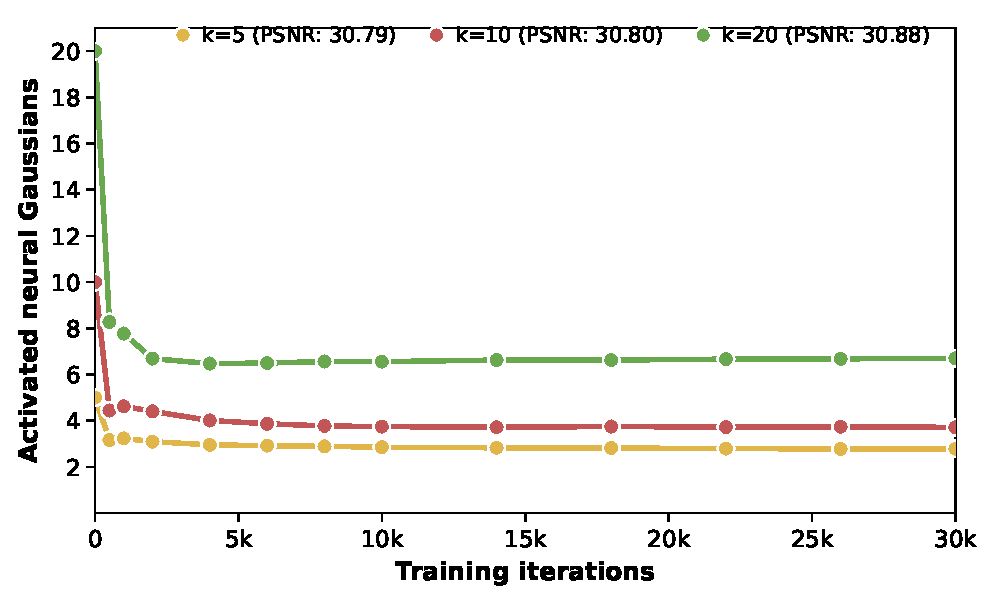
\includegraphics[width=0.98\linewidth]{figures/k_ablation.pdf}
  \caption{\textbf{Learning with different $k$ values} on Deep Blending
  \texttt{playroom}.
  $y$-axis: opacity-activated neural Gaussians per visible anchor.
  Despite $k\in\{5,10,20\}$, PSNR is essentially unchanged
  ($30.79$ / $30.80$ / $30.88$).}
  \label{fig:k-ablation}
\end{figure}
